\chapter{Deep Network}
\section{Deep learning}
Deep learning is a part of machine learning. It includes the methods based on learning data representation by allowing the computation on the models that are composed of multiple layers. Each layer extracts the representaion of the input data from the previous layer and computes a new presentation as the input for the next layer. In the hierachy of a model, the higher layers of representation enlarge aspects of the input that is important for discrimination and suppress irrelevant variations. Each level of representations is corresponding to the different level of abstraction. Deep learning methods work on a large dataset using the backpropagation algorithm to improve the result after each step. The methods of deep learning have effectively improved the results in classification problems, object recognition, speech recognition and other domains. 

In deep learning, a neural network is known as the popular method. This is a computing-system based on a collection of connected units (called neurons). Each connection (called synapse) between the neurons can transmit the signal from a neuron to another neuron. The receiving neuron processes the signal that it received, then it sends the resulting signal to another neuron connected to it. Neurons and synaptes may have the weights as learnabled variables, which can used to increase or decrease the strength of signal that it sends to next units. Normally, neurons are organized in layers with different kinds of transformation inside. The signal is travelled multiple times from the first layer (input layer) to the last layer (output layer).

\section{Neural network}
\subsection{Neural}
The basic components of the brain is a neuron. For the ordinary man, we have billion neurons in the human nervous system, and they are connected by the billion of synapses. Each neuron receives input signals from its dendrites and procedures output signals along its axon.\\[0.2cm]
In the computational model of a neuron, the signals travel along the axons interact multiplicatively with the dendrites of the other neuron based on the synaptic strength at the synapse. The synaptic strength are learnable and control the strength at influence or inhibitory of one neuron on another. In basic mode, the input signals are summed and compared with a threshold value. If the sum is greater than threshold value, the neuron can fire, sending a spike along its axon. Actually, we have many firing rate (called activation function) at a neuron, and the common choice of activation function is the \textbf{sigmoid funciont $\sigma$}, because it take a real-valued input and squashes it to range between 0 and 1. The image () show the model of a neuron:
\begin{figure}[h]
	\centering
	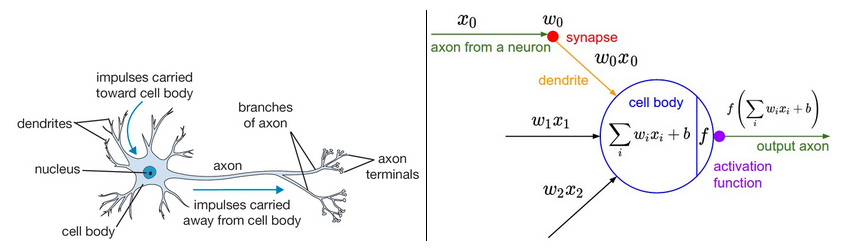
\includegraphics[scale=0.5]{images/neurons.png}
	\caption{A drawing of a biological neuron and its mathematical model}
	\label{fignneuron}
\end{figure}

Some activation functions which we can use:
\begin{itemize}
	\item \textbf{Sigmoid function}:
		\begin{equation}
			\sigma(x) = \frac{1}{1+e^{-x}}
		\end{equation}
	\item \textbf{Tanh}
		\begin{equation}
			tanh(x) = 2\sigma(2x) - 1
		\end{equation}
	\item \textbf{ReLU}
		\begin{equation}
			f(x) = max(0,x)
		\end{equation}
	\item \textbf{Maxout}:
		\begin{equation}
			f(w^Tx + b) = max({w_1}^Tx + b_1,{w_2}^Tx + b_2)
		\end{equation}
\end{itemize}
\section{The architecture of neural networks}
\begin{figure}[h]
	\centering
	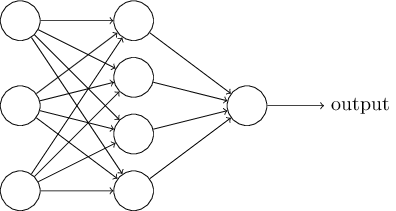
\includegraphics[scale=0.5]{images/neuron}
	\caption{A model of neural networks}
	\label{fignnnetworks}
\end{figure}
The image \ref{fignnnetworks} show a simple model of neural networks. The leftmost layer in this network is called the input layer, the rightmost layer is called the output layer. The neurons within the input layer are called input neurons, the neurons from output layer are called output neurons. The middle layer is called a hidden layer. The network in example \ref{fignnnetworks} has just a single hidden layer, but many networks have multiple hidden layers. When design the network, the input and the output are often straightforward. It means that the neural networks is designed where the output form one layer is used as the input to the next layer, there are no loops in the network, it always feed forward, never feed back (called feedforward networks).\\[0.2cm]
So, the neural network includes many layers are designed as an directred acyclic graph from the intput to the output layer. The output of previous layer is used as the input of the next layer. At each layer excepts the output layer, the output is indicated by a activation function (i.e loss, tanh,...). The size of a neural network can be to compute as the number of neurons, or the number of parameters.
\section{Deep network}
A deep neural network is a neural network with multiple layers between the input and the output layers. These layers are called hidden layers. Each layer tries to find the correct mathematical operator to turn its input into the next layer. The deep neural network forwards the data from the input layer to the output layer without looping back: The network creates the connections of neurons and assigns the ``weight" for each connection. At each layer, the weights and its input are multiplied and return an output. Further, an algorithm is used to adjust the weights so that make certain parameters more influential until it receives the correct mathematical manipulation on all dataset.

Besides the deep neural network, convolutional neural networks are other solutions for deep learning. It consists of an input, an output, as well as multiple hidden layers. The hidden layers of a CNN may be convolutional layers, pooling layers, normalization layers or fully connected layers. The layers of a CNN has neurons arranged in three dimensions of the input: \textit{width, height and depth} with learnable parameters.